% Template for PLoS
% Version 3.6 Aug 2022
%
% % % % % % % % % % % % % % % % % % % % % %
%
% -- IMPORTANT NOTE
%
% This template contains comments intended 
% to minimize problems and delays during our production 
% process. Please follow the template instructions
% whenever possible.
%
% % % % % % % % % % % % % % % % % % % % % % % 
%
% Once your paper is accepted for publication, 
% PLEASE REMOVE ALL TRACKED CHANGES in this file 
% and leave only the final text of your manuscript. 
% PLOS recommends the use of latexdiff to track changes during review, as this will help to maintain a clean tex file.
% Visit https://www.ctan.org/pkg/latexdiff?lang=en for info or contact us at latex@plos.org.
%
%
% There are no restrictions on package use within the LaTeX files except that no packages listed in the template may be deleted.
%
% Please do not include colors or graphics in the text.
%
% The manuscript LaTeX source should be contained within a single file (do not use \input, \externaldocument, or similar commands).
%
% % % % % % % % % % % % % % % % % % % % % % %
%
% -- FIGURES AND TABLES
%
% Please include tables/figure captions directly after the paragraph where they are first cited in the text.
%
% DO NOT INCLUDE GRAPHICS IN YOUR MANUSCRIPT
% - Figures should be uploaded separately from your manuscript file. 
% - Figures generated using LaTeX should be extracted and removed from the PDF before submission. 
% - Figures containing multiple panels/subfigures must be combined into one image file before submission.
% For figure citations, please use "Fig" instead of "Figure".
% See http://journals.plos.org/plosone/s/figures for PLOS figure guidelines.
%
% Tables should be cell-based and may not contain:
% - spacing/line breaks within cells to alter layout or alignment
% - do not nest tabular environments (no tabular environments within tabular environments)
% - no graphics or colored text (cell background color/shading OK)
% See http://journals.plos.org/plosone/s/tables for table guidelines.
%
% For tables that exceed the width of the text column, use the adjustwidth environment as illustrated in the example table in text below.
%
% % % % % % % % % % % % % % % % % % % % % % % %
%
% -- EQUATIONS, MATH SYMBOLS, SUBSCRIPTS, AND SUPERSCRIPTS
%
% IMPORTANT
% Below are a few tips to help format your equations and other special characters according to our specifications. For more tips to help reduce the possibility of formatting errors during conversion, please see our LaTeX guidelines at http://journals.plos.org/plosone/s/latex
%
% For inline equations, please be sure to include all portions of an equation in the math environment.  For example, x$^2$ is incorrect; this should be formatted as $x^2$ (or $\mathrm{x}^2$ if the romanized font is desired).
%
% Do not include text that is not math in the math environment. For example, CO2 should be written as CO\textsubscript{2} instead of CO$_2$.
%
% Please add line breaks to long display equations when possible in order to fit size of the column. 
%
% For inline equations, please do not include punctuation (commas, etc) within the math environment unless this is part of the equation.
%
% When adding superscript or subscripts outside of brackets/braces, please group using {}.  For example, change "[U(D,E,\gamma)]^2" to "{[U(D,E,\gamma)]}^2". 
%
% Do not use \cal for caligraphic font.  Instead, use \mathcal{}
%
% % % % % % % % % % % % % % % % % % % % % % % % 
%
% Please contact latex@plos.org with any questions.
%
% % % % % % % % % % % % % % % % % % % % % % % %

\documentclass[10pt,letterpaper]{article}
\usepackage[top=0.85in,left=2.75in,footskip=0.75in]{geometry}

% amsmath and amssymb packages, useful for mathematical formulas and symbols
\usepackage{amsmath,amssymb}

% Use adjustwidth environment to exceed column width (see example table in text)
\usepackage{changepage}

% textcomp package and marvosym package for additional characters
\usepackage{textcomp,marvosym}

% cite package, to clean up citations in the main text. Do not remove.
\usepackage{cite}

% Use nameref to cite supporting information files (see Supporting Information section for more info)
\usepackage{nameref,hyperref}

% line numbers
\usepackage[right]{lineno}

% ligatures disabled
\usepackage[nopatch=eqnum]{microtype}
\DisableLigatures[f]{encoding = *, family = * }

% color can be used to apply background shading to table cells only
\usepackage[table]{xcolor}

% array package and thick rules for tables
\usepackage{array}

% create "+" rule type for thick vertical lines
\newcolumntype{+}{!{\vrule width 2pt}}

% create \thickcline for thick horizontal lines of variable length
\newlength\savedwidth
\newcommand\thickcline[1]{%
  \noalign{\global\savedwidth\arrayrulewidth\global\arrayrulewidth 2pt}%
  \cline{#1}%
  \noalign{\vskip\arrayrulewidth}%
  \noalign{\global\arrayrulewidth\savedwidth}%
}

% \thickhline command for thick horizontal lines that span the table
\newcommand\thickhline{\noalign{\global\savedwidth\arrayrulewidth\global\arrayrulewidth 2pt}%
\hline
\noalign{\global\arrayrulewidth\savedwidth}}


% Remove comment for double spacing
%\usepackage{setspace} 
%\doublespacing

% Text layout
\raggedright
\setlength{\parindent}{0.5cm}
\textwidth 5.25in 
\textheight 8.75in

% Bold the 'Figure #' in the caption and separate it from the title/caption with a period
% Captions will be left justified
\usepackage[aboveskip=1pt,labelfont=bf,labelsep=period,justification=raggedright,singlelinecheck=off]{caption}
\renewcommand{\figurename}{Fig}

% Use the PLoS provided BiBTeX style
\bibliographystyle{plos2015}

% Remove brackets from numbering in List of References
\makeatletter
\renewcommand{\@biblabel}[1]{\quad#1.}
\makeatother



% Header and Footer with logo
\usepackage{lastpage,fancyhdr,graphicx}
\usepackage{epstopdf}
%\pagestyle{myheadings}
\pagestyle{fancy}
\fancyhf{}
%\setlength{\headheight}{27.023pt}
%\lhead{\includegraphics[width=2.0in]{PLOS-submission.eps}}
\rfoot{\thepage/\pageref{LastPage}}
\renewcommand{\headrulewidth}{0pt}
\renewcommand{\footrule}{\hrule height 2pt \vspace{2mm}}
\fancyheadoffset[L]{2.25in}
\fancyfootoffset[L]{2.25in}
\lfoot{\today}

%% Include all macros below

\newcommand{\lorem}{{\bf LOREM}}
\newcommand{\ipsum}{{\bf IPSUM}}

%% END MACROS SECTION

%% use-defined citations & references colors
\definecolor{ceruleanblue}{rgb}{0.16, 0.32, 0.75}
\hypersetup{
    colorlinks=true,
    citecolor=ceruleanblue,
    linkcolor=ceruleanblue,
    urlcolor=ceruleanblue
}
%% end user-defined colors

%% user-defined math definitions
\def\calR{\mathcal{R}}
\def\bbN{\mathbb{N}}
\def\bbR{\mathbb{R}}
\def\bbZ{\mathbb{Z}}
\DeclareMathOperator*{\diag}{diag}
\DeclareMathOperator*{\argmin}{argmin}
\newcommand{\Argmin}[1]{\underset{#1}{\argmin\ }}
\def\sumN{\sum_{i=1}^n}
\newcommand{\fr}[1]{\frac{1}{#1}}
\newcommand{\lr}[1]{\left(#1\right)}
\newcommand{\norm}[1]{\left\lVert #1 \right\rVert}
\def\Dxkk{D^{(x,k+1)}}
%% END math definitions

%% user-defined reference structures
\renewcommand{\eqref}[1]{Eq~(\ref{#1})}
\renewcommand{\chapterautorefname}{Chapter}
\renewcommand{\sectionautorefname}{Section}
%% END reference structures

\begin{document}
\vspace*{0.2in}

% Title must be 250 characters or less.
\begin{flushleft}
{\Large
\textbf\newline{Adaptively temporal evolution of reproduction number estimation with trend filtering} % Please use "sentence case" for title and headings (capitalize only the first word in a title (or heading), the first word in a subtitle (or subheading), and any proper nouns).
}
\newline
% Insert author names, affiliations and corresponding author email (do not include titles, positions, or degrees).
\\
Jiaping Liu\textsuperscript{1},
Zhenglun Cai\textsuperscript{2},
Daniel J. McDonald\textsuperscript{1*}
\\
\bigskip
\textbf{1} Department of Statistics, The University of British Columbia, Vancouver, British Columbia, Canada

\textbf{2} ? 
\\
\bigskip

% Insert additional author notes using the symbols described below. Insert symbol callouts after author names as necessary.
% 
% Remove or comment out the author notes below if they aren't used.
%
% Primary Equal Contribution Note
%\Yinyang These authors contributed equally to this work.

% Additional Equal Contribution Note
% Also use this double-dagger symbol for special authorship notes, such as senior authorship.
%\ddag These authors also contributed equally to this work.

% Current address notes
%\textcurrency Current Address: Department of Statistics, The University of British Columbia, Vancouver, British Columbia, Canada % change symbol to "\textcurrency a" if more than one current address note
% \textcurrency b Insert second current address 
% \textcurrency c Insert third current address

% Deceased author note
%\dag Deceased

% Group/Consortium Author Note
%\textpilcrow Membership list can be found in the Acknowledgments section.

% Use the asterisk to denote corresponding authorship and provide email address in note below.
* daniel@stat.ubc.ca

\end{flushleft}
% Please keep the abstract below 300 words
\section*{Abstract}
aaa

% Please keep the Author Summary between 150 and 200 words
% Use first person. PLOS ONE authors please skip this step. 
% Author Summary not valid for PLOS ONE submissions.   
\section*{Author summary}
xxx

\linenumbers

% Use "Eq" instead of "Equation" for equation citations.
\section*{Introduction}
\label{sec:intro}

% Reproduction number describes the contagiousness or transmissibility of infectious agents
The basic reproduction number ($\calR_0$), defined as the expected number of secondary infections caused by an infected individual in a completely susceptible population, is a fundamental indicator of epidemiological transmissibility \cite{diekmann1990definition,dietz1993estimation,fine1993herd}. The reproduction number provides a threshold such that when $\calR_0<1$, the infection dies out gradually, which is known as the \textit{disease-free equilibrium}, and when $\calR_0>1$, the \textit{endemic equilibrium} is asymptotically achieved, i.e., the infection is always present \cite{diekmann1990definition,delamater2019complexity,brauer2019mathematical}. Basic reproduction numbers reflect the potential sizes of a pandemic and suggests the scale of epidemic prevention measures such as the proportion of a population that should be vaccinated \cite{anderson1982directly,anderson1985vaccination,heffernan2005perspectives,delamater2019complexity}. 

% R_t 
\textbf{Effective reproduction numbers} ($\calR_t$ at time $t$, also called as, instantaneous reproduction numbers) differ from the basic reproduction numbers by relaxing the assumption of a completely susceptible population. It only varies from $\calR_0$ by a constant scale ($x$ such that $\calR_t=\calR_0 x$) -- the proportion of susceptible individuals over the population though, it is able to explain more factors that may influence the spread of infectious diseases such as the changes of transmission rates due to interventions. Therefore, effective reproduction numbers are more interpretable in reality. We focus on effective reproduction numbers throughout this section and call them as reproduction numbers for simplicity.

% the necessity of modeling R_t 
Reproduction number reflects a biological reality though, it is rarely measured directly. The observations in practice are the infective cases. Mathematical biologists and theoretic epidemiologists have proposed complicated mathematical models to estimate this metric using various assumptions. For this reason, the estimated reproduction number of a pathogen varies. Different estimations in turn suggest different ways to control the further tendency of reproduction numbers. For example, if reproduction numbers are assumed to be affected by human-human interaction over time, controlling the parameters influencing human-human contact rate may eventually lead to a reduction of the reproduction numbers. Hence, mathematical modelling requires the domain expertise for specific infectious diseases dynamics to set the assumptions. % varying along with local sociobehavioral and environmental circumstances.

% apply PTF on Rt estimation
Reproduction numbers at discretized timepoints of a given population have a natural structure of line graphs, where each node representing a reproduction number at a timepoint is connected to its previous and next nodes in time along a line. Temporal evolution of reproduction numbers considers the progression of reproduction numbers that occurs over time through different temporal intervals. Here, we apply Poisson trend filtering on line graphs to model the temporal evolution of reproduction numbers, where various degrees can reflect various temporal intervals that the progression occurs. 

% an existing approach to model R_0
A group of epidemiological models are compartmental models. They establish the epidemic transmission process by creating compartments with labels and connecting them by directed edges. A simple compartmental model -- for example, \textit{Susceptible-Infectious-Susceptible} (SIS) model -- divides the population ($N$) into two compartments for susceptible cases ($S$) and infectious cases ($I$) respectively and connects them in serial as $S\to I\to S$. It only focuses on susceptible individuals. Each directed edge corresponds to a ratio of transmission (say, $\alpha,\beta$ respectively). In such models, reproduction numbers are defined as functions of the estimated transmission parameters and the numbers of compartments or population, e.g., $\hat{\calR}_0=\hat{\beta} N/\hat{\alpha}$ in the SIS models \cite{brauer2019mathematical}, as by-products. Compartmental models usually solve ordinary differential equations (ODE) systems for transmission numbers (e.g., $\alpha,\beta$ in the SIS model). A disadvantage of such parametric models is that they are less flexible than nonparametric models and the number of parameters to be estimated grows along with the increase of compartments in practice, which results in a growing computational complexity. Since the epidemic mechanism depends highly on the contexts, e.g., if a latency period exists or not, such models are lack of generalizability. Moreover, data of high quality are not always available for all compartments especially when there is a pandemic outbreak that results in a sudden shortage of resources in collecting daily new infections. %the sensitivity to low-quality data and the complex computation

% the approach we focus
To overcome these limitations of compartmental models, there is an alternative branch of approaches estimating reproduction numbers directly without expressing them as functions of other transmission parameters. Such approaches only require the knowledge of the infected counts and the distributional assumption on serial interval, which is a duration of onsets of symptoms between a primary case and secondary cases. A remarkable point is that serial interval is a widely used metric to approximate the generation time, defined as the duration between the infection of a transmission pair -- an infector and an infectee. Generation time is theoretically better to measure the transmission duration than serial interval; however, it is also generally unobservable and more tricky to estimate. In this section, we will focus on one of the direct approaches to estimate reproduction number $\calR_t$. 

\section*{Framework}


\subsection*{Bayesian hierarchical model} 

Let observed daily new infections on day $i$ be $y_i \in \bbN$. 
Cori et al. \cite{cori2013new} suggested that incident confirmed cases on day $i$ followed Poisson distributions with the expectations being the product of the reproduction numbers and the weighted sum of confirmed cases prior to day $i$. The weighted previous confirmed cases here reflected the contagious mechanism that a current confirmed case was infected several days ago. The weight corresponding to a previous day represented the probability that the current cases were infected on the very day. The probabilities were approximated by \textit{serial interval functions}. %Serial intervals are usually unobservable, so assumptions of distributions are required. %Serial interval is also called as generation interval or generation time, when the infectiousness profile after symptoms is independent of the incubation period \cite{cori2013new}. 
%They suggested a Bayesian framework such that maximizing the posteriori of reproduction number given a gamma prior and Poisson infection counts. 
Abry et al. \cite{abry2020spatial} extended this approach by introducing a (second-order) temporal regularization and a spatial regularization of reproduction rates and proposed to solve it as an optimization problem. % such that minimizing the log-likelihood of the posteriori of the Poisson parameters given their priori and observed infections. 
Pascal et al. \cite{pascal2022nonsmooth} further introduced robustness against outliers.

In this project, we focus on the temporal evolution of reproduction numbers and extend it from a second-order divided difference to all orders ($1,2,3,...$). We propose a locally adaptive estimator measuring the time series of reproduction numbers. Compared to existing mathematical models for reproduction number estimation, this estimator is more flexible in the order of temporal evolution of reproduction numbers and also locally adaptive so that it captures the local changes such as the initiation of effective control measures. More specifically, it regularizes the similarity among reproduction numbers across a chosen number of neighboring time points and segments the curvature of the reproduction numbers such that there are more jumpiness in some subregions and more smoothness in others. We find the proposed estimator is identical to the univariate Poisson trend filtering estimator with a slight modification. We assume the serial interval function is known and approximated it by Gamma distributions following previous studies \cite{cori2013new,thompson2019improved,abry2020spatial,pascal2022nonsmooth}.
%The epidemiology evolution mechanism suggests a hierarchical framework that posteriori of reproduction number depends on its prior and the distribution of confirmed cases. 

\subsection*{Poisson trend filtering estimator} %Proximal optimization

We assume that the count of observed daily new infections at time $i$ ($y_i$) follows a Poisson distribution with the natural parameter being the effective reproduction number ($\calR_i > 0$) scaled by the weighted sum of previous daily counts, denoted by $w_i \geq 0$ for $i=1,\cdots,n$. %(Denote $\calR:=\calR_t$ hereafter.) 
Let $\theta:=\log(\calR) \in \mathbb{R}^n$, and then $w\circ \calR = w\circ e^{\theta}$, $\log(w\circ \calR) = \log(w) + \theta$, where $e^{a}, \log(a)$ apply to a vector $a$ elementwise. We further regularize the smoothness of the reproduction number using the $\ell_1$ norm of the divided difference of the natural logarithm of $\calR$, which is real-valued. 

The extended Poisson trend filtering (PTF) on univariate cases is then defined as:
\begin{equation} \label{eq:rt-ptf}
    \begin{split}
        \hat{\theta} &:= \Argmin{\theta\in\bbR^n} \fr{n}\sumN -y_i \theta_i + w_i e^{\theta_i} + \lambda \norm{D^{(k+1)} \theta}_1, \\
        \hat{\calR} &:= e^{\hat{\theta}},
    \end{split}
\end{equation}
where $D^{k+1} \in \bbZ^{(n-k-1)\times n}$ is the $k$-th order divided difference matrix with $k=0,1,2,3,\cdots$. Define $D^{(k+1)}$ recursively as $D^{(k+1)} := D^{(1)} D^{(k)}$, where $D^{(1)}\in\bbN^{(n-k-1)\times (n-k)}$ and $D^{(1)}$ is a banded matrix with $(-1,1)$ on the columns $(i,i+1)$ for each row $i=1,...,n-k-1$. Define $D^{(0)} := I_n$. An exponential transformation is applied to the PTF estimator to get the estimated reproduction number.
%
For unequally spaced signals, replace $D^{(k+1)}$ by $D^{(x,k+1)}$ with weights $x\in \mathbb{R}^n$ (which are signal locations). Define $D^{(x,k+1)}$ recursively as $D^{(x,k+1)} := D^{(1)}\cdot X^k \cdot D^{(x,k)}, $
where $$X^k := \diag \lr{\frac{k}{x_{k+1} - x_1}, \frac{k}{x_{k+2} - x_2}, \cdots, \frac{k}{x_n - x_{n-k}} }$$ is a diagonal matrix depending on the order $k$.

We use Gamma distribution to estimate the serial interval function, i.e., weights of the previous daily infections. On day $i$, the weights of previous counts $y_1,...,y_{i-1}$ have corresponding coefficients (weights) $\Phi_1,..,\Phi_{i-1}$, which are probabilities of gamma distribution with prespecified parameters $(\alpha,\beta)$ corresponding to specific quartiles. The weight corresponding to $\calR_i$ is $w_i = \sum_{j=1}^{\tau_{\Phi}} \Phi_j y_{i-j}$, where $\tau_{\Phi}$ is a chosen period of infection.


\subsection*{Proximal Newton method} %Specialized ADMM for `generalized' Poisson trend filtering on lines

We use proximal Newton method to solve the proximal optimization problem in \eqref{eq:rt-ptf}. During each outer Newton-based iteration, we use specialized ADMM \cite{ramdas2016fast} to solve the problem in the inner loop. %Both algorithms follow similar procedures as in \autoref{sec:generic-algo}, but with a specialized substitution. %Details are provided in Appendix \ref{sec:spec-algo}. 
%in linearized ADMM and proximal Newton method proposed in Section \ref{sec:spec-algo} to solve the problem in \eqref{eq:rt-ptf}.
% explain the precondition if necessary: .. refer to \cite{chambolle2011first} used in \cite{pascal2022nonsmooth}


The outer Newton-based iteration solves the following problems at time $t+1$:
\begin{align} \label{spec-prox}
  \theta_+^t &= \mathrm{prox}_{W_w^t,\Dxkk} \lr{c_w^{t}}, \\
  \theta^{t+1} &= \theta_+^t + \gamma^{t+1} \lr{\theta_+^t - \theta^t},
\end{align}
where $W_w^t := \diag \lr{w\circ e^{\theta^t}}\in \bbR^{n\times n}$ and $c_w^t := y^t\circ w^{-1}\circ e^{-\theta^t} + \theta^t - \boldsymbol{1}$.% where $a^{-1}$ is an elementwise operator for vector $a$.

% defer to the section of Simulation: 
%\subsection*{Range of $\lambda$} 
%Find the maximum lambda such that the estimated $\theta$ does not fall into the null space of the divided difference matrix.


% Results and Discussion can be combined.
\section*{Applications and results}

Implementation of the proximal Newton method is provided in the \texttt{R} package \href{https://dajmcdon.github.io/rtestim/}{\texttt{rtestim}}. 

\subsection*{Covid-19 cases}

% introduce data & hyperparameter setup
We implement the proposed model on the Covid-19 confirmed cases in British Columbia (B.C.) as of May 18, 2023 reported by B.C. Conservation Data Centre. We choose the gamma distribution with shape $2.5$ and scale $2.5$ to approximate the serial interval function.

\begin{figure}[tb]
    \centering
    %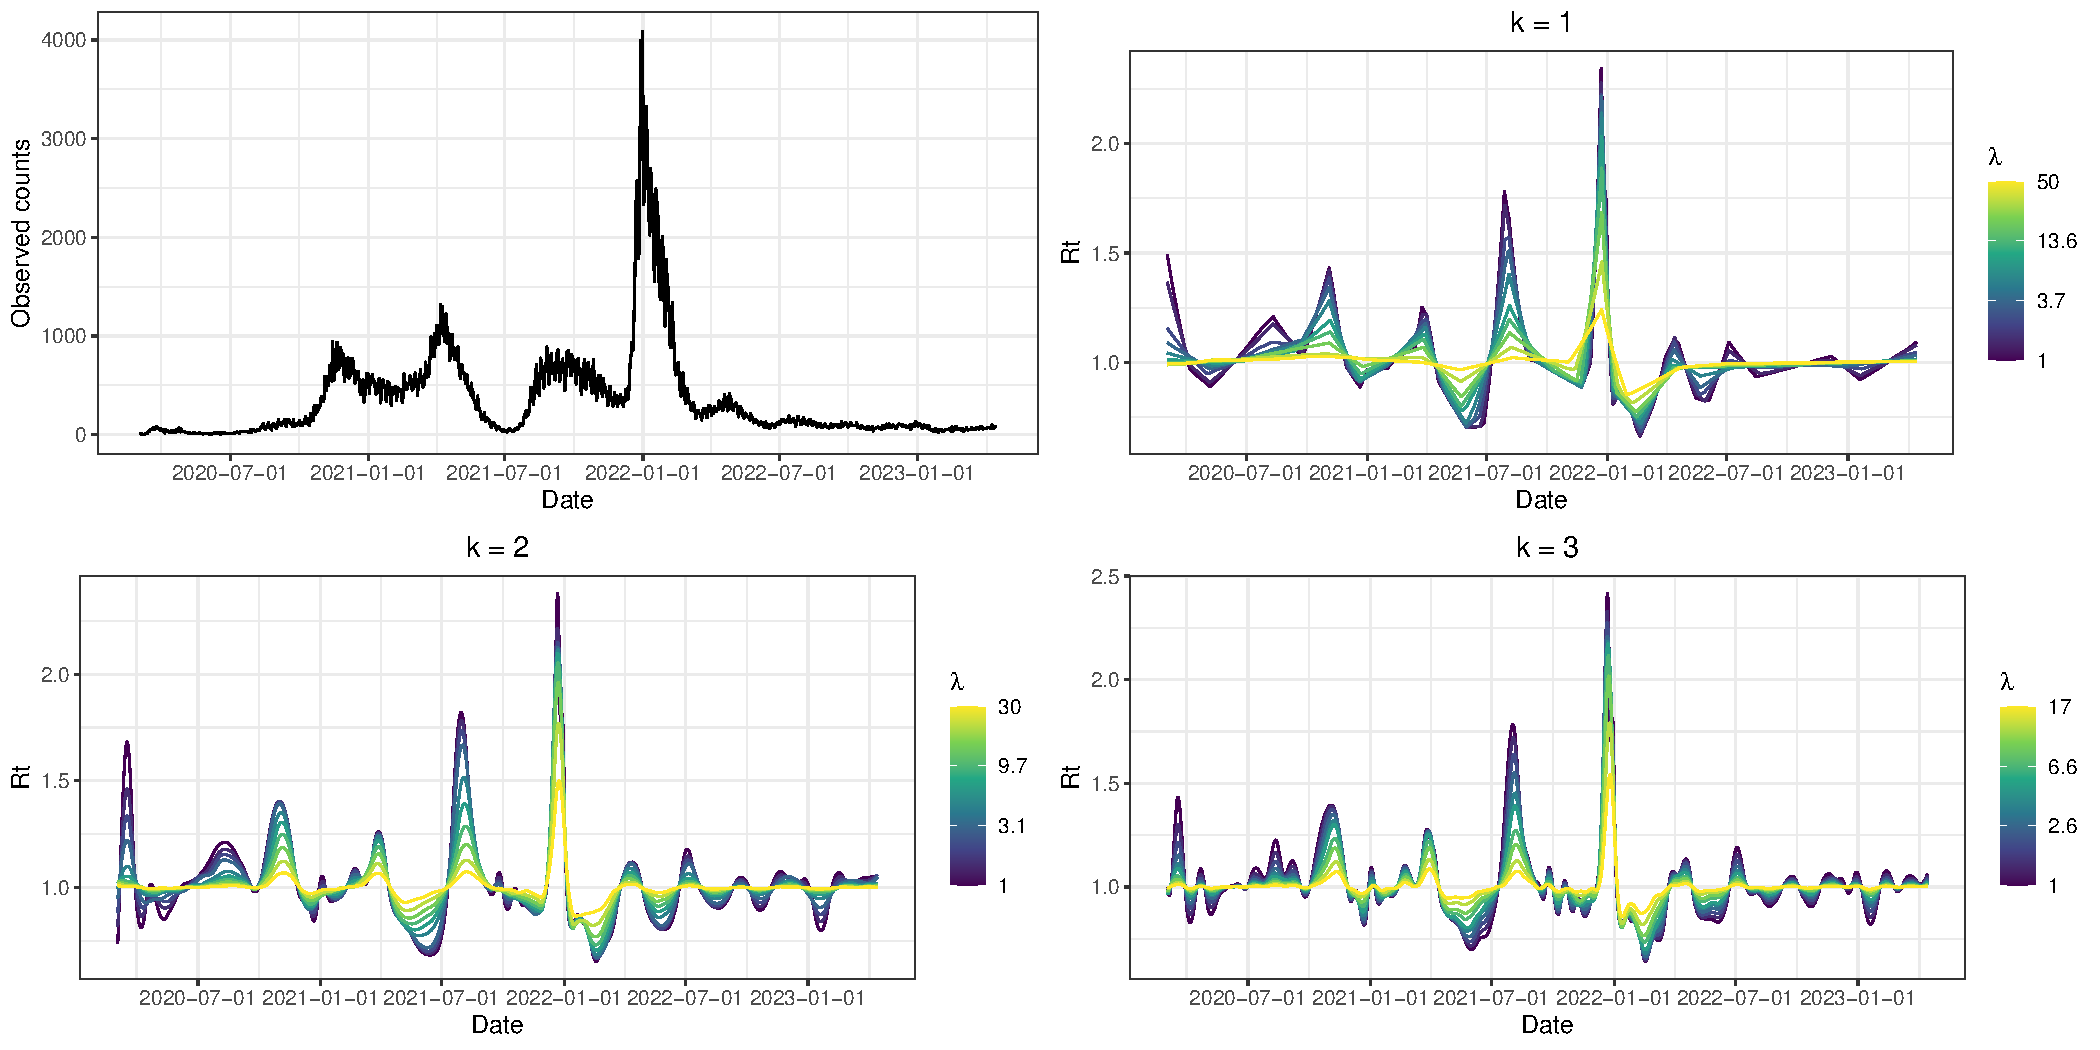
\includegraphics[width=0.99\linewidth]{fig/covid19fig.pdf}
    \caption{Covid19 daily confirmed counts between March 1st, 2020 and April 15th, 2023 in British Columbia, Canada. The top left panel displays the time trend of the observed infectious cases. The top right, bottom left and bottom right panels illustrated the estimated reproduction numbers ($\calR_t$) using the Poisson trend filtering (in \eqref{eq:rt-ptf}) with degrees $k=1,2,3$ respectively.} 
\end{figure}

% interpret figures -- across all lambdas
Considering the temporal evolutions of neighboring $3, 4, 5$ reproduction numbers, the estimated reproduction numbers of Covid-19 in British Columbia (displayed in the top right, bottom left, and bottom right panels in Fig 1 respectively) are always lower than $2.5$, which means that two distinct infected individuals can on average infect less than five other individuals in the population. The three degrees of the temporal evolution (across all regularization levels $\lambda$) all yield similar results that $\hat{\calR}_t$ achieves the highest peak around the end of 2021 and reaches the lowest trough shortly thereafter. Throughout the estimated curves, the peaks and troughs of the reproduction numbers roughly come prior to the following growths and decays of confirmed cases respectively.

The reproduction numbers are relatively unstable before April 1st, 2022.
The highest peak coincides with the emergence and globally spread of the Omicron variant. The estimated reproduction numbers are apparently below the threshold $1$ during two time periods -- roughly from April 1st, 2021 to July 1st, 2021 and from January 1st, 2022 to April 1st, 2022. The first trough of $\hat{\calR}_t$ coincides with the first authorization for use of Covid-19 vaccines in British Columbia. The second trough shortly after the greatest peak may credit to many aspects, including self-isolation of the infected individuals and application of the second shot of Covid-19 vaccines. 
Since around April 1st, 2022, the reproduction numbers stay stable (at around $1$) and the infected cases stay low. 

% for different lambda
Greater regularization levels (i.e., larger $\lambda$s) result in smoother estimated curves. Smoother curves (e.g., the yellow curve in the top right panel in Fig 1) suggest that the estimated reproduction numbers are around $1$ during most time periods; however, they may not be appropriate to interpret the reality. More wiggly curves better reflect the fluctuation of $\calR_t$, but sometimes fail to highlight the significant peaks or troughs. The tuning parameter $\lambda$ needs to be chosen corresponding to the information in practice for a better interpretation.

\section*{Discussion}

% advantages
The proposed methodology provides a locally adaptive estimator using Poisson trend filtering on univariate data for capturing the heterogeneous smoothness of effective reproduction numbers given time series of infective observations in a given region. This is a nonparametric regression model which can be written as convex optimization(minimization) problem. Minimizing the distance (averaged KL divergence per coordinate) between the estimators and observations guarantees the data fidelity; minimizing a certain order of divided differences between each pair of neighboring parameters regularizes the smoothness. The $\ell_1$ regularization introduces sparsity to the divided differences, which leads to heterogeneous smoothness within certain periods of time. The homogeneous smoothness within a time period can be either performed by a constant reproduction number, or a constant rate of changes, or a constant graphical curvature depending on the prescribed degree ($k=0,1,2$ respectively). %The estimator is uniquely defined due to its strict convexity. 

The property of local adaptivity is useful for interpreting seasonal outbreaks. Given a properly chosen degree of polynomials, for example, the growth rate in a seasonal outbreak can be distinguished from the counterparts in un-seasonal outbreak periods at the beginning of the outbreak, which will alert epidemiologists to propose sanitary policies to prevent the progressing outbreak. The effective reproduction numbers can be estimated afterwards to check the efficiency of the sanitary policies referring to whether they are below the threshold, their tendencies of reduction, or their graphical curvatures.

% how about regional evolution?
%A limitation is that it only takes the temporal evolution within a single region into account, and fails to consider the spatial connection or spatial-temporal evolution among regions. 
A potential future work is to extend the proposed model to analyze spatio-temporal infectious data. Such data have the inherit graphical structure such that temporal evolution within a region can be connected by lines (as time series) and spatial connection (of cross-sectional data) can be constructed by graphs where each pair of neighboring regions is linked by an edge. Moreover, the spatio-temporal evolution, i.e., the effects of previous infectious data of one region on current infections of neighboring regions, can be measured, for example, by linking the node of region $a$ at time $t-1$ to another node of region $b$ at time $t$. 
%Through this way, different orders of spatial and temporal evolutions can be manually manipulated. 
In this case, we can directly apply Poisson trend filtering on graphs with minor adjustment. %A remarkable note is that the edge lengths need to be made comparable across temporal and regional connections.


% assumptions and limitations
Our proposed model provides a natural way to deal with missing data, e.g., on weekends and holidays. Since the edge lengths of the line graphs can be adjusted, we can manually increase the length between two observations if there are missing data in between so that the influence of a previous observation is reduced correspondingly. Moreover, the $\ell_1$ penalty introduces sparsity, and thus, makes the estimators less sensitive to outliers compared to $\ell_2$ regularization. 
It is remarkable that our focus is to provide a mathematical model for epidemiologists to use, rather than to focus on a specific disease. In addition, more specialized methodologies are needed for the diseases with relatively long incubation periods (e.g., HIV and HBV). 
% used for acute diseases with short serial intervals 


\section*{Conclusion}

xxx


\section*{Supporting information}

% Include only the SI item label in the paragraph heading. Use the \nameref{label} command to cite SI items in the text.
\paragraph*{S1 Fig.}
\label{S1_Fig}
{\bf Covid-19 figure.} Covid-19 cases in BC and the estimated reproduction numbers.

\paragraph*{S2 Fig.}
\label{S2_Fig}
{\bf Lorem ipsum.} Maecenas convallis mauris sit amet sem ultrices gravida. Etiam eget sapien nibh. Sed ac ipsum eget enim egestas ullamcorper nec euismod ligula. Curabitur fringilla pulvinar lectus consectetur pellentesque.

\paragraph*{S1 File.}
\label{S1_File}
{\bf Lorem ipsum.}  Maecenas convallis mauris sit amet sem ultrices gravida. Etiam eget sapien nibh. Sed ac ipsum eget enim egestas ullamcorper nec euismod ligula. Curabitur fringilla pulvinar lectus consectetur pellentesque.

\paragraph*{S1 Video.}
\label{S1_Video}
{\bf Lorem ipsum.}  Maecenas convallis mauris sit amet sem ultrices gravida. Etiam eget sapien nibh. Sed ac ipsum eget enim egestas ullamcorper nec euismod ligula. Curabitur fringilla pulvinar lectus consectetur pellentesque.

\paragraph*{S1 Appendix.}
\label{S1_Appendix}
{\bf Lorem ipsum.} Maecenas convallis mauris sit amet sem ultrices gravida. Etiam eget sapien nibh. Sed ac ipsum eget enim egestas ullamcorper nec euismod ligula. Curabitur fringilla pulvinar lectus consectetur pellentesque.

\paragraph*{S1 Table.}
\label{S1_Table}
{\bf Lorem ipsum.} Maecenas convallis mauris sit amet sem ultrices gravida. Etiam eget sapien nibh. Sed ac ipsum eget enim egestas ullamcorper nec euismod ligula. Curabitur fringilla pulvinar lectus consectetur pellentesque.

\section*{Acknowledgments}
Cras egestas velit mauris, eu mollis turpis pellentesque sit amet. Interdum et malesuada fames ac ante ipsum primis in faucibus. Nam id pretium nisi. Sed ac quam id nisi malesuada congue. Sed interdum aliquet augue, at pellentesque quam rhoncus vitae.

\nolinenumbers

% Either type in your references using
% \begin{thebibliography}{}
% \bibitem{}
% Text
% \end{thebibliography}
%
% or
%
% Compile your BiBTeX database using our plos2015.bst
% style file and paste the contents of your .bbl file
% here. See http://journals.plos.org/plosone/s/latex for 
% step-by-step instructions.
% 
\begin{thebibliography}{10}

  \bibitem{diekmann1990definition}
  Diekmann O, Heesterbeek JAP, Metz JA.
  \newblock On the definition and the computation of the basic reproduction ratio
    R 0 in models for infectious diseases in heterogeneous populations.
  \newblock Journal of mathematical biology. 1990;28:365--382.
  
  \bibitem{dietz1993estimation}
  Dietz K.
  \newblock The estimation of the basic reproduction number for infectious
    diseases.
  \newblock Statistical methods in medical research. 1993;2(1):23--41.
  
  \bibitem{fine1993herd}
  Fine PE.
  \newblock Herd immunity: history, theory, practice.
  \newblock Epidemiologic reviews. 1993;15(2):265--302.
  
  \bibitem{delamater2019complexity}
  Delamater PL, Street EJ, Leslie TF, Yang YT, Jacobsen KH.
  \newblock Complexity of the basic reproduction number (R0).
  \newblock Emerging infectious diseases. 2019;25(1):1.
  
  \bibitem{brauer2019mathematical}
  Brauer F, Castillo-Chavez C, Feng Z.
  \newblock Mathematical models in epidemiology. vol.~32.
  \newblock Springer; 2019.
  
  \bibitem{anderson1982directly}
  Anderson RM, May RM.
  \newblock Directly transmitted infections diseases: control by vaccination.
  \newblock Science. 1982;215(4536):1053--1060.
  
  \bibitem{anderson1985vaccination}
  Anderson RM, May RM.
  \newblock Vaccination and herd immunity to infectious diseases.
  \newblock Nature. 1985;318(6044):323--329.
  
  \bibitem{heffernan2005perspectives}
  Heffernan JM, Smith RJ, Wahl LM.
  \newblock Perspectives on the basic reproductive ratio.
  \newblock Journal of the Royal Society Interface. 2005;2(4):281--293.
  
  \bibitem{cori2013new}
  Cori A, Ferguson NM, Fraser C, Cauchemez S.
  \newblock A new framework and software to estimate time-varying reproduction
    numbers during epidemics.
  \newblock American journal of epidemiology. 2013;178(9):1505--1512.
  
  \bibitem{abry2020spatial}
  Abry P, Pustelnik N, Roux S, Jensen P, Flandrin P, Gribonval R, et~al.
  \newblock Spatial and temporal regularization to estimate COVID-19 reproduction
    number R (t): Promoting piecewise smoothness via convex optimization.
  \newblock Plos one. 2020;15(8):e0237901.
  
  \bibitem{pascal2022nonsmooth}
  Pascal B, Abry P, Pustelnik N, Roux S, Gribonval R, Flandrin P.
  \newblock Nonsmooth convex optimization to estimate the Covid-19 reproduction
    number space-time evolution with robustness against low quality data.
  \newblock IEEE Transactions on Signal Processing. 2022;70:2859--2868.
  
  \bibitem{thompson2019improved}
  Thompson RN, Stockwin JE, van Gaalen RD, Polonsky JA, Kamvar ZN, Demarsh PA,
    et~al.
  \newblock Improved inference of time-varying reproduction numbers during
    infectious disease outbreaks.
  \newblock Epidemics. 2019;29:100356.
  
  \bibitem{ramdas2016fast}
  Ramdas A, Tibshirani RJ.
  \newblock Fast and flexible admm algorithms for trend filtering.
  \newblock Journal of Computational and Graphical Statistics.
    2016;25(3):839--858.
  
\end{thebibliography}
  

%\bibliography{ptf}
\end{document}
